%%%%%%%%%%%%%%%%%%%%%%%%%%%%%%%%%%%%%%%%%%%%%%%%%%%%
\section{Context Learning}\label{sec:context_learning}
%%%%%%%%%%%%%%%%%%%%%%%%%%%%%%%%%%%%%%%%%%%%%%%%%%%%

\newcommand{\success}{\mbox{\emph{succ}}}
\newcommand{\failure}{\mbox{\emph{fail}}}

With the classical BDI programming framework extended with decision trees and a
probabilistic plan selection scheme, we are now ready to develop mechanisms for
learning context decision trees and hopefully improving over time the selection
of plans based on experience.
% %
To that end, in this section, we explore two approaches for learning the context
condition of plans.




Recall that our ultimate objective is to learn which plans are best for achieving
a particular goal event in the various world states that may ensue. Given that,
in this work, we have no measure of cost for plans,\footnote{This could also be a
useful addition, but is not part of standard BDI programming languages.} a good
plan for a given world state is simply one which (usually) succeeds in such
state. In order to learn the context decision tree for a plan, the agent keeps
track of previous experiences she has had when running the plan in question. More
precisely, if a plan $P$ is tried in world state $w$ with certain outcome $o \in
\{\success,\failure\}$, the agent may record the tuple $\tuple{w,o}$ as part of
the training set for plan $P$.
% %
Interestingly, while it is always meaningful to record successful executions,
some failures may not be worth recording. Based on this observation, we shall
develop and compare two different algorithms that differ on how past experiences
are taken into account by the agent. Before then, though, let us explain better
this issue by means of an example.
 

\begin{figure}[t]
\begin{center}
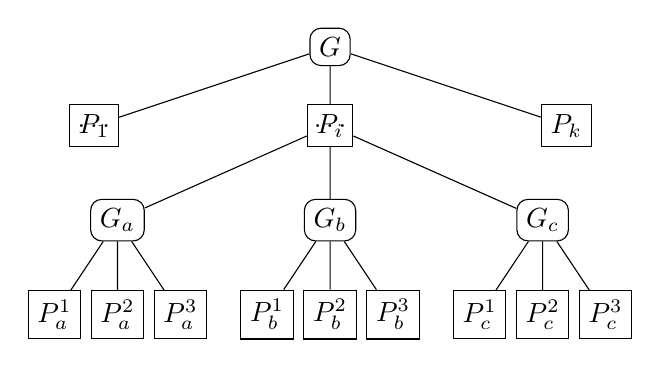
\begin{tikzpicture}[level distance=1.2cm]

\tikzstyle{planbox}=[draw]
\tikzstyle{goalbox}=[draw,rounded corners]

\tikzstyle{level 1}=[sibling distance=3cm,level distance=1cm] 
\tikzstyle{level 2}=[sibling distance=2.7cm,level distance=1.2cm] 
\tikzstyle{level 3}=[sibling distance=.8cm]

\node[goalbox,yshift=1cm,solid] (T) {$G$}
   child {node[planbox] (P1) {$P_1$}}
   	child[solid] {node[planbox] (1) (Pi) {$P_i$}
      child {node[goalbox] {$G_a$}
		child {node[planbox] {$P_a^1$}}
		child {node[planbox] {$P_a^2$}}
		child {node[planbox] {$P_a^3$}}
	}
      child {node[goalbox] {$G_b$}
		child {node[planbox] {$P_b^1$}}
		child {node[planbox] {$P_b^2$}}
		child {node[planbox] {$P_b^3$}}
	}
      child {node[goalbox] {$G_c$}
		child {node[planbox] {$P_c^1$}}
		child {node[planbox] {$P_c^2$}}
		child {node[planbox] {$P_c^3$}}
	}
	}
   child {node[planbox] {$P_k$}};

\node[right of=P1,xshift=-1cm]  {$\ldots$};
\node[right of=Pi,xshift=-1cm]  {$\ldots$};

\end{tikzpicture}

% \begin{tikzpicture}[level distance=1.2cm]
% 
% \tikzstyle{planbox}=[draw]
% \tikzstyle{goalbox}=[draw,rounded corners]
% 
% \tikzstyle{level 2}=[sibling distance=2.8cm] 
% \tikzstyle{level 3}=[sibling distance=3.4cm]
% \tikzstyle{level 4}=[sibling distance=1.8cm]
% \tikzstyle{level 5}=[sibling distance=1cm]
% 
% \node[goalbox,dashed] (G) {$G$}
% child[dashed] { node[planbox,dashed] (top) {$P$}
% child[dashed] {node[goalbox,below left of=top,yshift=1cm,solid] (T) {$G_0$}
%    child[solid] {node[planbox,label=below:$\longrightarrow$] (1) {$P_1$}
%       child {node[goalbox] (11) {$G_{1}$}
% 		child {node[planbox] {$P_3$}}
% 		child {node[planbox] {$P_4$}}
% 	}
%       child {node[goalbox] (12) {$G_{2}$}
% 		child {node[planbox] {$P_5$}}
% 		child {node[planbox] {$P_6$}}
% 	}
%       child {node[goalbox] (13) {$G_{3}$}
% 		child {node[planbox] {$P_7$}}
% 	}
%       }
%    child[solid] {node[planbox] (2) {$P_2$}
%       child {node[goalbox] (22) {$G_{3}$}
% 	child {node[planbox] {$P_8$}}
% 	child {node[planbox] {$P_9$}}
% 	}
%    }
% }
% };
% 
% \draw (T) -- (1) node (aux1) [coordinate,midway]{};
% \draw (T) -- (2) node (aux2) [coordinate,midway]{};
% \draw (aux1) .. controls +(0.3,-0.3) and +(-0.3,-0.3).. (aux2)
% 			node[midway,above] {OR};
% 
% % \draw (1) -- (11) node (aux21) [coordinate,midway]{};
% % \draw (1) -- (12) node (aux23) [coordinate,midway]{};
% % \draw (aux21) .. controls +(0.25,-0.25) and +(-0.25,-0.25).. (aux23)
% % 			node[midway,above] {AND};
% 
% % \node[below left of=T,text width=2cm,xshift=-3cm] (label)
% % 		{$P_i$: plan \\ $G_i$: goals \\ $SG_i$: sub-goals};
% \end{tikzpicture}

\end{center}
% \caption{Goal-plan tree hierarchy. Rounded boxes stand for event goals; rectangles for plans.}
\caption{Goal-plan tree hierarchy $\T_3$. Rounded boxes stand for event goals; rectangles for
plans. Top-level goal $G$ as $k$ relevant plans, each of them with a goal-plan
tree structure below them as shown for plan $P_i$.}
%
% \caption{Goal-plan tree hierarchy $\T_3$. Rounded boxes stand for event goals; rectangles for
% plans. Leaf plans are assumed to directly succeed or fail when executed in the environment, and
% are marked accordingly. 
% %
% An edge with a label $\times n$ states that there are $n$ edges of such type (e.g.,  goal $G$ has
% $5$ relevant plans). Indexes are used to represent different goals/plans under such labeled edges.
% For instance, below $P_1$, the indexes are understood as $i \in \{1,2\}$, $j \in \{1,\ldots,3\}$,
% and $k \in \{2,\ldots,5\}$.
% %
% To succeed, an agent should execute $6$ working plans, namely, $P_{1111}^1$, $P_{1112}^1$, and 
% $P_{1113}^1$ to resolve goal $G_1^1$, and $P_{1211}^1$, $P_{1212}^1$, and 
% $P_{1213}^1$ to resolve goal $G_1^2$.}
\label{fig:T3}
\end{figure}



Consider the example in Figure \ref{fig:T3}.
% %
Suppose that in some execution, plan $P_\ell$, for some $\ell \in \{1,\ldots,k\}$
is selected in order to resolve top-goal $G$ in some world state $w_1$. The plan
involves, in turn, the successful resolution of three sequential goals $G_a$,
$G_b$, and finally $G_c$. Suppose further that subgoal $G_1$ has been resolved
successfully, yielding new state $w_2$, and that plan $P_b^2$ has been chosen
next to try and achieve the second subgoal $G_b$.
% %
Suppose next that the execution of plan $P_b^2$, which may involve more subgoals,
happens to \emph{fail}. As we have no failure recovery, this will immediately
cause goal $G_b$ itself to fail, and recursively will cause failure at each level
until top-level goal $G$ itself fails.
% %
Clearly, the failure should be recorded in the decision tree of the plan where
the failure originated, namely, plan $P_b^2$. However, it is not so clear, as
will be discussed next, whether the failure should also be recorded in the
decision trees for plans higher up in the hierarchy, for example, in plan
$P_\ell$ (the one selected to address $G$).


In order to discuss further which data should be recorded where, we define the
notion of an \textit{active execution trace}, as a sequence of the form
$G_0[P_0:w_0] \cdot G_1[P_1:w_1] \cdot \ldots \cdot G_n[P_n:w_n]$, which
represents the sequence of currently active goals, along with the plans which
have been selected to achieve each of them, and the world state in which the
selection was made---plan $P_i$ has been selected in world state $w_i$ in order
to achieve the $i$-th active subgoal $G_i$.
% %
In our example, the trace at the moment of failure is as follows:
\[ \lambda=G[P_\ell:w_1] \cdot G_b[P_b^2:w_2]. \]


So, when the final goal of $\lambda$ fails, namely $G_b$, it is clear that the
decision tree of the plan being used to achieve that goal ought to be updated, in
the example, a failure should be recorded for the world state $w_2$ for the
decision tree attached to plan $P_2^b$.  Although it may be the case that the
plan usually succeeds in the situation in which it was chosen, and failure is
simply due to some non-determinism (or in the general case, actions of other
agents, interactions, etc.), there is no way to determine this and the learning
process will eventually recognise such cases as ``noise.''
% %
However, should the decision trees of plans associated with earlier goals in
$\lambda$ (e.g., the one for $P_\ell$) be updated?  The point is that it is
conceivable that the failure of goal $G_b$ could have been avoided, had an
alternative plan, say $P_b^1$, been chosen instead. If this is the case, then
recording a failure against plan $P_\ell$ would not not be justified.
% %
Informally, one could argue that it is best to wait before recording failures
against a plan until one is reasonably confident that subsequent choices down the
goal-plan tree hierarchy were ``well informed.'' In order words, if the agent
knows that the plan selection for goal $G_b$ was as good and informed as
possible, then recording the failure for world $w_1$ in plan $P_\ell$ would
also be justified.


\newcommand{\procedurefont}[1]{\mathsf{#1}}
\newcommand{\StableGoal}{\procedurefont{StableGoal}}
\newcommand{\RecordTrace}{\procedurefont{RecordFailedTrace}}
\newcommand{\RecordWorldDT}{\procedurefont{RecordWorldDT}}

% The judgment as to whether the decisions made were sufficiently ``well
% informed'', is however not a trivial one. We develop an algorithm that
% makes the decision as to whether to record a failure, based on a
% notion of stability, where a plan is considered to be stable for a
% particular world state $w$ if the rate of success of $P$ in $w$ is
% changing below a certain threshold, $\epsilon$. We also allow
% specification of a minimum number of execution experiences for $P$ in
% $w$, in order to have the change of rate of success be sufficiently
% meaningful. A goal is considered to be stable for world state $w$ if
% all its relevant plans are stable for $w$.

% Stephane replaced the paragraph. I thought it was better to present
% the notion of stability first, then to say that stability is what we
% consider as well informed, and then introduce the algorithm.

The judgment as to whether the decisions made were sufficiently ``well
informed,'' is however not a trivial one.  A plan $P$ is considered to
be \emph{stable} for a particular world state $w$ if the rate of
success of $P$ in $w$ is changing below a certain threshold,
$\epsilon$.
% comments by Stephane 
% o I guess here, something more correct would be that the rate of
% success of P in the leaf node of the decision tree that contains w.
% I'm not sure it is worth precising.
% o is the rate of change computing over a window of the last n use of
% the plan?
%stephane adds:
If the rate of success does not change much after some
observations, we can start to build confidence about it.
% end add
We also allow specification of a minimum number of execution
experiences for $P$ in $w$, in order to have the change of rate of
success be sufficiently meaningful. A goal is considered to be stable
for world state $w$ if all its relevant plans are stable for $w$.  We
consider that the decision of recording a failure for a plan is ``well
informed'' when the goal it is being chosen for is stable.  We use a function
$\StableGoal(G,w,k,\epsilon)$ which returns true iff goal $G$ is
considered \textit{stable} for world state $w$, under minimal
% stephane changed from minimal execution traces to number of
% execution, I was getting confused whether there was a concpet of
% "minimal trace". I thought it would be clearer like this.
 number of executions and change of success rate thresholds $k \geq 0$
 and $0 < \epsilon \leq 1$, respectively.

\begin{algorithm}\caption{$\RecordTrace(\lambda,k,\epsilon)$}\label{algo:record_failed_exec}
KwData{$\lambda=G_0[P_0:w_0] \cdot \ldots \cdot G_n[P_n:w_n]$; $k\geq0$; $\epsilon > 0$}
\medskip

$\RecordWorldDT(P_n,w_n,failure)$

If{$[\StableGoal(G_n,w_n,k,\epsilon) \land |\lambda|>1]$} {
	tcp{\small decision for $G_n$ was informed}
	$\lambda' \longleftarrow G_0[P_0:w_0] \cdot \ldots \cdot G_{n-1}[P_{n-1}:w_{n-1}]$
	$\RecordTrace(\lambda',k,\epsilon)$
}
\end{algorithm}

The algorithm starts by assimilating the failure in the last plan
$P_n$ in the trace, by recording the world $w_n$ in which $P_n$ was
started as a ``failure'' case.
% Stephane modified here to mention that there must be a previous node
% here, which explains the |\lambda| > 1
If there is a previous node in the trace (i.e. for the plan $P_{n-1}$
which required achievement of the failed goal $G_n$) and the choice of
executing plan $P_n$ to achieve goal $G_n$ was indeed an informed one
(that is, goal $G_n$ was stable for $w_n$), the procedure is repeated
for the previous node in the trace.  If, on the other hand, the last
goal $G_n$ in the trace is not considered stable enough, the procedure
terminates and no more data is assimilated.
%
It follows then that, in order to update the decision tree of a certain
plan, it has to be the case that the (failed) decisions taken during
the plan execution must have been informed enough.
The closer to 0 $\epsilon$ is, and the higher $k$ is, the more
conservative the agent will be in considering its decisions well
informed. With $\epsilon$ = 1 and k = 0 we obtain a more standard
learning approach where all information is accumulated, and the
assumption is made that faulty information will eventually disappear
as noise.

So, in the remaining of the paper, we shall compare two cases. The first we call
aggressive concurrent learning (\CL) and is exactly the more traditional approach where all data is
assimilated by the learner, that is, we take $\epsilon = 1$ and $k = 0$.
% \footnote{Those values imply that plans/goals are always deemed stable.}
%Stephane questions: is it really k=0? Shouldn'it be at least 1?
The second we call bottom-up learning (\BUL), and we use $\epsilon = 0.3$ and
$k = 3$.
%according to Scott's email.
We explore these two approaches on some programs with different
structures  and discuss the results.
